\documentclass[a4paper,10pt]{article}
\usepackage{wasysym}
\usepackage{enumitem}
\usepackage{forloop}
\usepackage{graphicx}

\newcommand{\creq}[1]{
    [\textbf{C\arabic{cReqNum}: #1}]%
    \addtocounter{cReqNum}{10}%
}

\newcommand{\Qq}[1]{#1}

\newcommand{\QO}{$\Box$}% or: $\ocircle$

\newcounter{qr}
\newcommand{\Qrating}[1]{\QO\forloop{qr}{1}{\value{qr} < #1}{---\QO}}

\newcommand{\Qline}[1]{\noindent\rule{#1}{0.6pt}}

\newcounter{ql}
\newcommand{\Qlines}[1]{\forloop{ql}{0}{\value{ql}<#1}{\vskip0em\Qline{\linewidth}}}

\newenvironment{Qlist}{%
\renewcommand{\labelitemi}{\QO}
\begin{itemize}[leftmargin=1.5em,topsep=-.5em]
}{
\end{itemize}
}

\newlength{\qt}
\newcommand{\Qtab}[2]{
\setlength{\qt}{\linewidth}
\addtolength{\qt}{-#1}
\hfill\parbox[t]{\qt}{\raggedright #2}
}

\newcommand{\Qitem}[2][]{
\begin{enumerate}[topsep=2pt,leftmargin=2.8em]
\item[\textbf{C\arabic{cReqNum}#1.}] #2
\addtocounter{cReqNum}{10}
\end{enumerate}
}

\title{Product Specification: blender-hand-drawn-npr}

\begin{document}

\maketitle
\tableofcontents


\section{Purpose}

This document defines the functional and non-functional requirements of the System. 
These requirements will form the basis of all User Stories.

Section \ref{projectbrief} is quoted verbatim from the Project Brief and form the initial Customer requirements.
Further Customer requirements elicited from subsequent meetings and a questionnaire are presented in Section \ref{customermeetings} and \ref{customerquestionnaire} respectively.

Requirements within this document are identified in \textbf{bold} and given a unique requirement ID.

\newpage
\section{Initial Requirements}
\subsection{Project Brief} \label{projectbrief}
\newcounter{cReqNum}
\setcounter{cReqNum}{10}

This project will look at augmenting 3D rendering software to produce \creq{high-quality} \creq{scientific} \creq{3D} surfaces with \creq{pseudo hand drawn} appearance. The project will focus on extending the \creq{Blender} [blender.org] renderer to produce these graphs, most likely via \creq{Python} scripting.

Traditional hand drawn plots (see below) are able to \creq{reveal structure} in 3D surfaces that is often lost in modern renders. Although modern renders have accurate light transport models, they are designed for photo realism rather than to reveal the structure of surfaces. This is particularly relevant when producing figures for \creq{reproduction}, which must be \creq{clear} and might only be \creq{monochrome}.

Traditional artists developed techniques to \creq{reveal shading} and surface features. The aim of this project will be to develop a system to produce high quality images \creq{automatically}, according to a specification provided by a user (e.g. \creq{line-only}, \creq{highlight creases}, \creq{no lighting}).

\subsection{Customer Meetings} \label{customermeetings}

\subsubsection{18-June-2018: Kick-Off (Week 1)}

\begin{itemize}
\item A \creq{blender add-on} is to be developed which will produce images of hand-drawn appearance.
\item \creq{Animation will not be supported}, i.e. \creq{temporal cohesion is not a concern}.
\item \creq{3D model will be the input}.
\item \creq{Vector SVG will be the output}.
\item Drawing style shall reveal surface details and \creq{shape}, \creq{regions of high-curvature} etc.
\item \creq{A specific drawing style shall be chosen}, although \creq{system design shall be flexible enough to add additional styles} at a later date.
\item \creq{No requirement to reveal surface texture}.
\item \creq{Lines shall be scaled according to distance of the camera from the object}.
\item A nice feature to have could be to \creq{mark areas of the model which must be rendered with a line/pattern} (e.g. to draw attention to specific areas of interest, or to allow non-deterministic output).
\end{itemize}

\subsubsection{25-June-2018: Weekly (Week 2)}

\begin{itemize}
\item Focus is on black and white images, however \creq{it may be useful to look at limited use of colour (2-3 colours max)}.
\end{itemize}


\newpage
\section{Questionnaire} \label{questionnaire}
\subsection{Non-Functional Requirements}
\subsubsection{Clarification of Initial Requirements}

\Qitem{\Qq{Ref C10, define the term ``high-quality''.} \Qlines{4}}
\Qitem{\Qq{Ref C50, state the minimum Blender version number to support.} \Qlines{1}}
\Qitem{\Qq{Ref C80, ``reproduction'' method is assumed to be photocopying. Please clarify if otherwise.} \Qlines{2}}
\Qitem{\Qq{Ref C100, ``monochrome'' is assumed to mean strokes will be rendered in a single colour, rather than in tones of a single colour. Please clarify if otherwise.} \Qlines{2}}
\Qitem{\Qq{Ref C120 and C190, it is assumed the the User will configure a Blender scene with a 3D surface mesh, including creation and positioning of a camera and any required lighting. This will be the starting point for interaction with the add-on. Please clarify if otherwise.} \Qlines{4}}
\Qitem{\Qq{Ref C200, state the minimum SVG version number to support.} \Qlines{1}}
\Qitem{\Qq{Ref C230, development will focus on producing stroke-based illustrations in the Pen-and-Ink style, which aligns with requirements C10, C40, C70, C80, C90, C100, C110, C210 and C220. If another illustration style is thought to be better suited, please state it here.} \Qlines{2}}

\subsubsection{Additional Requirements}

\Qitem{\Qq{Which operating systems shall be supported? Please also indicate minimum version numbers.}
\begin{Qlist}
\item Windows: \Qline{4cm}
\item Linux: \Qline{4cm}
\item MacOS: \Qline{4cm}
\item Other: \Qline{10cm}
\end{Qlist}
}
\Qitem{Please rate the relative importance of each of the following characteristics:
\begin{itemize}
\item Functionality \Qtab{3cm}{least important \Qrating{6} most important}
\item Reliability \Qtab{3cm}{least important \Qrating{6} most important}
\item Usability \Qtab{3cm}{least important \Qrating{6} most important}
\item Efficiency \Qtab{3cm}{least important \Qrating{6} most important}
\item Maintainability \Qtab{3cm}{least important \Qrating{6} most important}
\item Portability \Qtab{3cm}{least important \Qrating{6} most important}
\end{itemize}
}
\Qitem{\Qq{If there are other functional non-requirements not captured by the sections above, please state them here.} \Qlines{10}}

\subsection{Functional Requirements}
\subsubsection{Clarification of Initial Requirements}

\Qitem{\Qq{Ref C130, ``line-only'' is assumed to mean only the object outline/silhouette will be rendered. Please clarify if otherwise.} \Qlines{2}}
\Qitem{\Qq{Ref C140, ``highlight creases'' is assumed to mean only edges whose neighbouring faces meet at an angle greater than a User-defined value will be rendered. Please clarify if otherwise.} \Qlines{2}}
\Qitem{\Qq{Ref C150, ``no lighting'' is assumed to mean only geometric data (or world data such as ambient occlusion) would be used to determine the placement of feature-highlighting strokes. Please clarify if otherwise.} \Qlines{2}}

\subsubsection{Additional Requirements}

\Qitem{\Qq{C130, C140 and C150 cover some basic modes of operation. Are any other modes of operation required? If so, please state them here.} \Qlines{4}}
\Qitem{\Qq{Ref C270, selection of faces or edges will either be via the existing selection tools available in the Blender wireframe view, or by ``painting'' areas using the Blender Grease Pencil. If one particular method is more desirable, or if another method is required, please state it here.} \Qlines{4}}
\Qitem{\Qq{If there are other functional requirements not captured by the sections above, please state them here.} \Qlines{10}}


\newpage
\section{Initial Design}

\subsection{System Architecture}

\subsection{Domain Model}


\newpage
\section{User Stories}

TBA.


\newpage
\subsection{Coverage Matrix}

\begin{figure}[h]
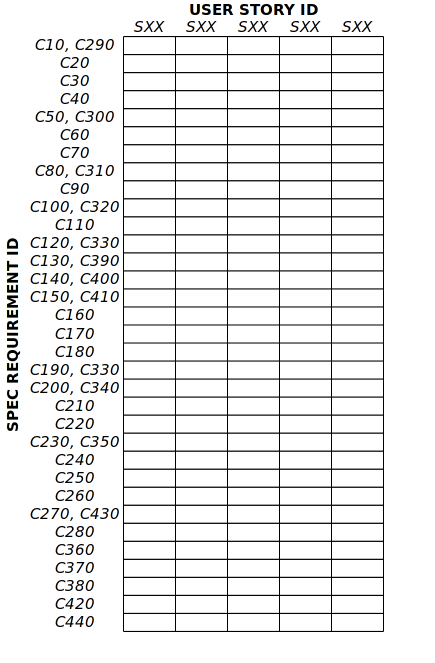
\includegraphics[width=8cm]{coverage_matrix}
\centering
\end{figure}

\end{document}